\chapter{Литературный обзор} \label{chapt1}

\section{Структура и свойства гексагонального  нитрида бора} \label{sect1_1}
Примерами классических квази-2D-структур являются слоистые кристаллы.
Изучение таких кристаллов началось еще в конце сороковых годов
двадцатого века~\cite{Wallace1947} и продолжается по сей день.
Наиболее интересными представителями таких систем являются кристаллы
гексагонального нитрида бора и графита. В настоящей работе исследовался
именно гексагональный нитрид бора.
% \subsection{Кристаллическая структура} \label{sect1_3_1}


Нитрид бора существует в различных модификациях: ромбоэдрический нитрид
бора(g-BN), кубический нитрид бора(c-BN)~\cite{Litvinov1998},
вюрцитный нитрид бора($\omega$-BN) и гексагональный нитрид бора
(h-BN) рис.~\ref{pic:BN_forms}(a). Также нитрид бора может существовать в виде нанотрубок~\cite{YZhi2009}
и фуллеренов.
\begin{figure}[!ht]
\center{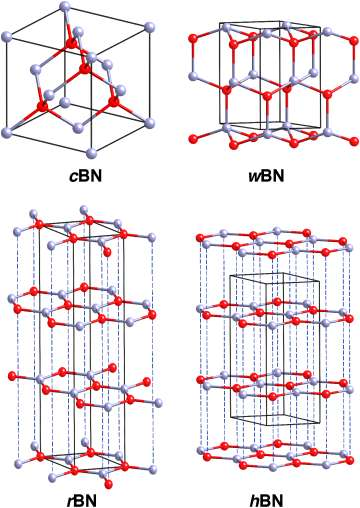
\includegraphics[width=0.6\linewidth]{BN_forms.png}}
\caption{Модификации нитрида бора(а). 
Слои гексагонального нитрида бора(b).}
\label{pic:BN_forms}
\end{figure}


Гексагональный нитрид бора является наиболее стабильной формой нитрида
бора. Как и графит, h-BN представляет собой слоистую структуру~\cite{
Neumann1995,Doni1969}. Каждый слой состоит из гексагонов, в вершинах
которых находятся, чередуя друг друга, атомы бора и азота рис.~\ref{pic:BN_forms}(b). Слои h-BN расположены таким образом, что атомы азота
находятся над атомами бора и наоборот. Результатом такого расположения слоев 
является дополнительное межплоскостное электростатическое взаимодействие
между атомами азота и бора. Постоянные решетки гексагонального нитрида
бора составляют $a=b=2.50\si{\angstrom}$~\cite{Paszkowicz2001}. 
\begin{figure}[!ht]
\center{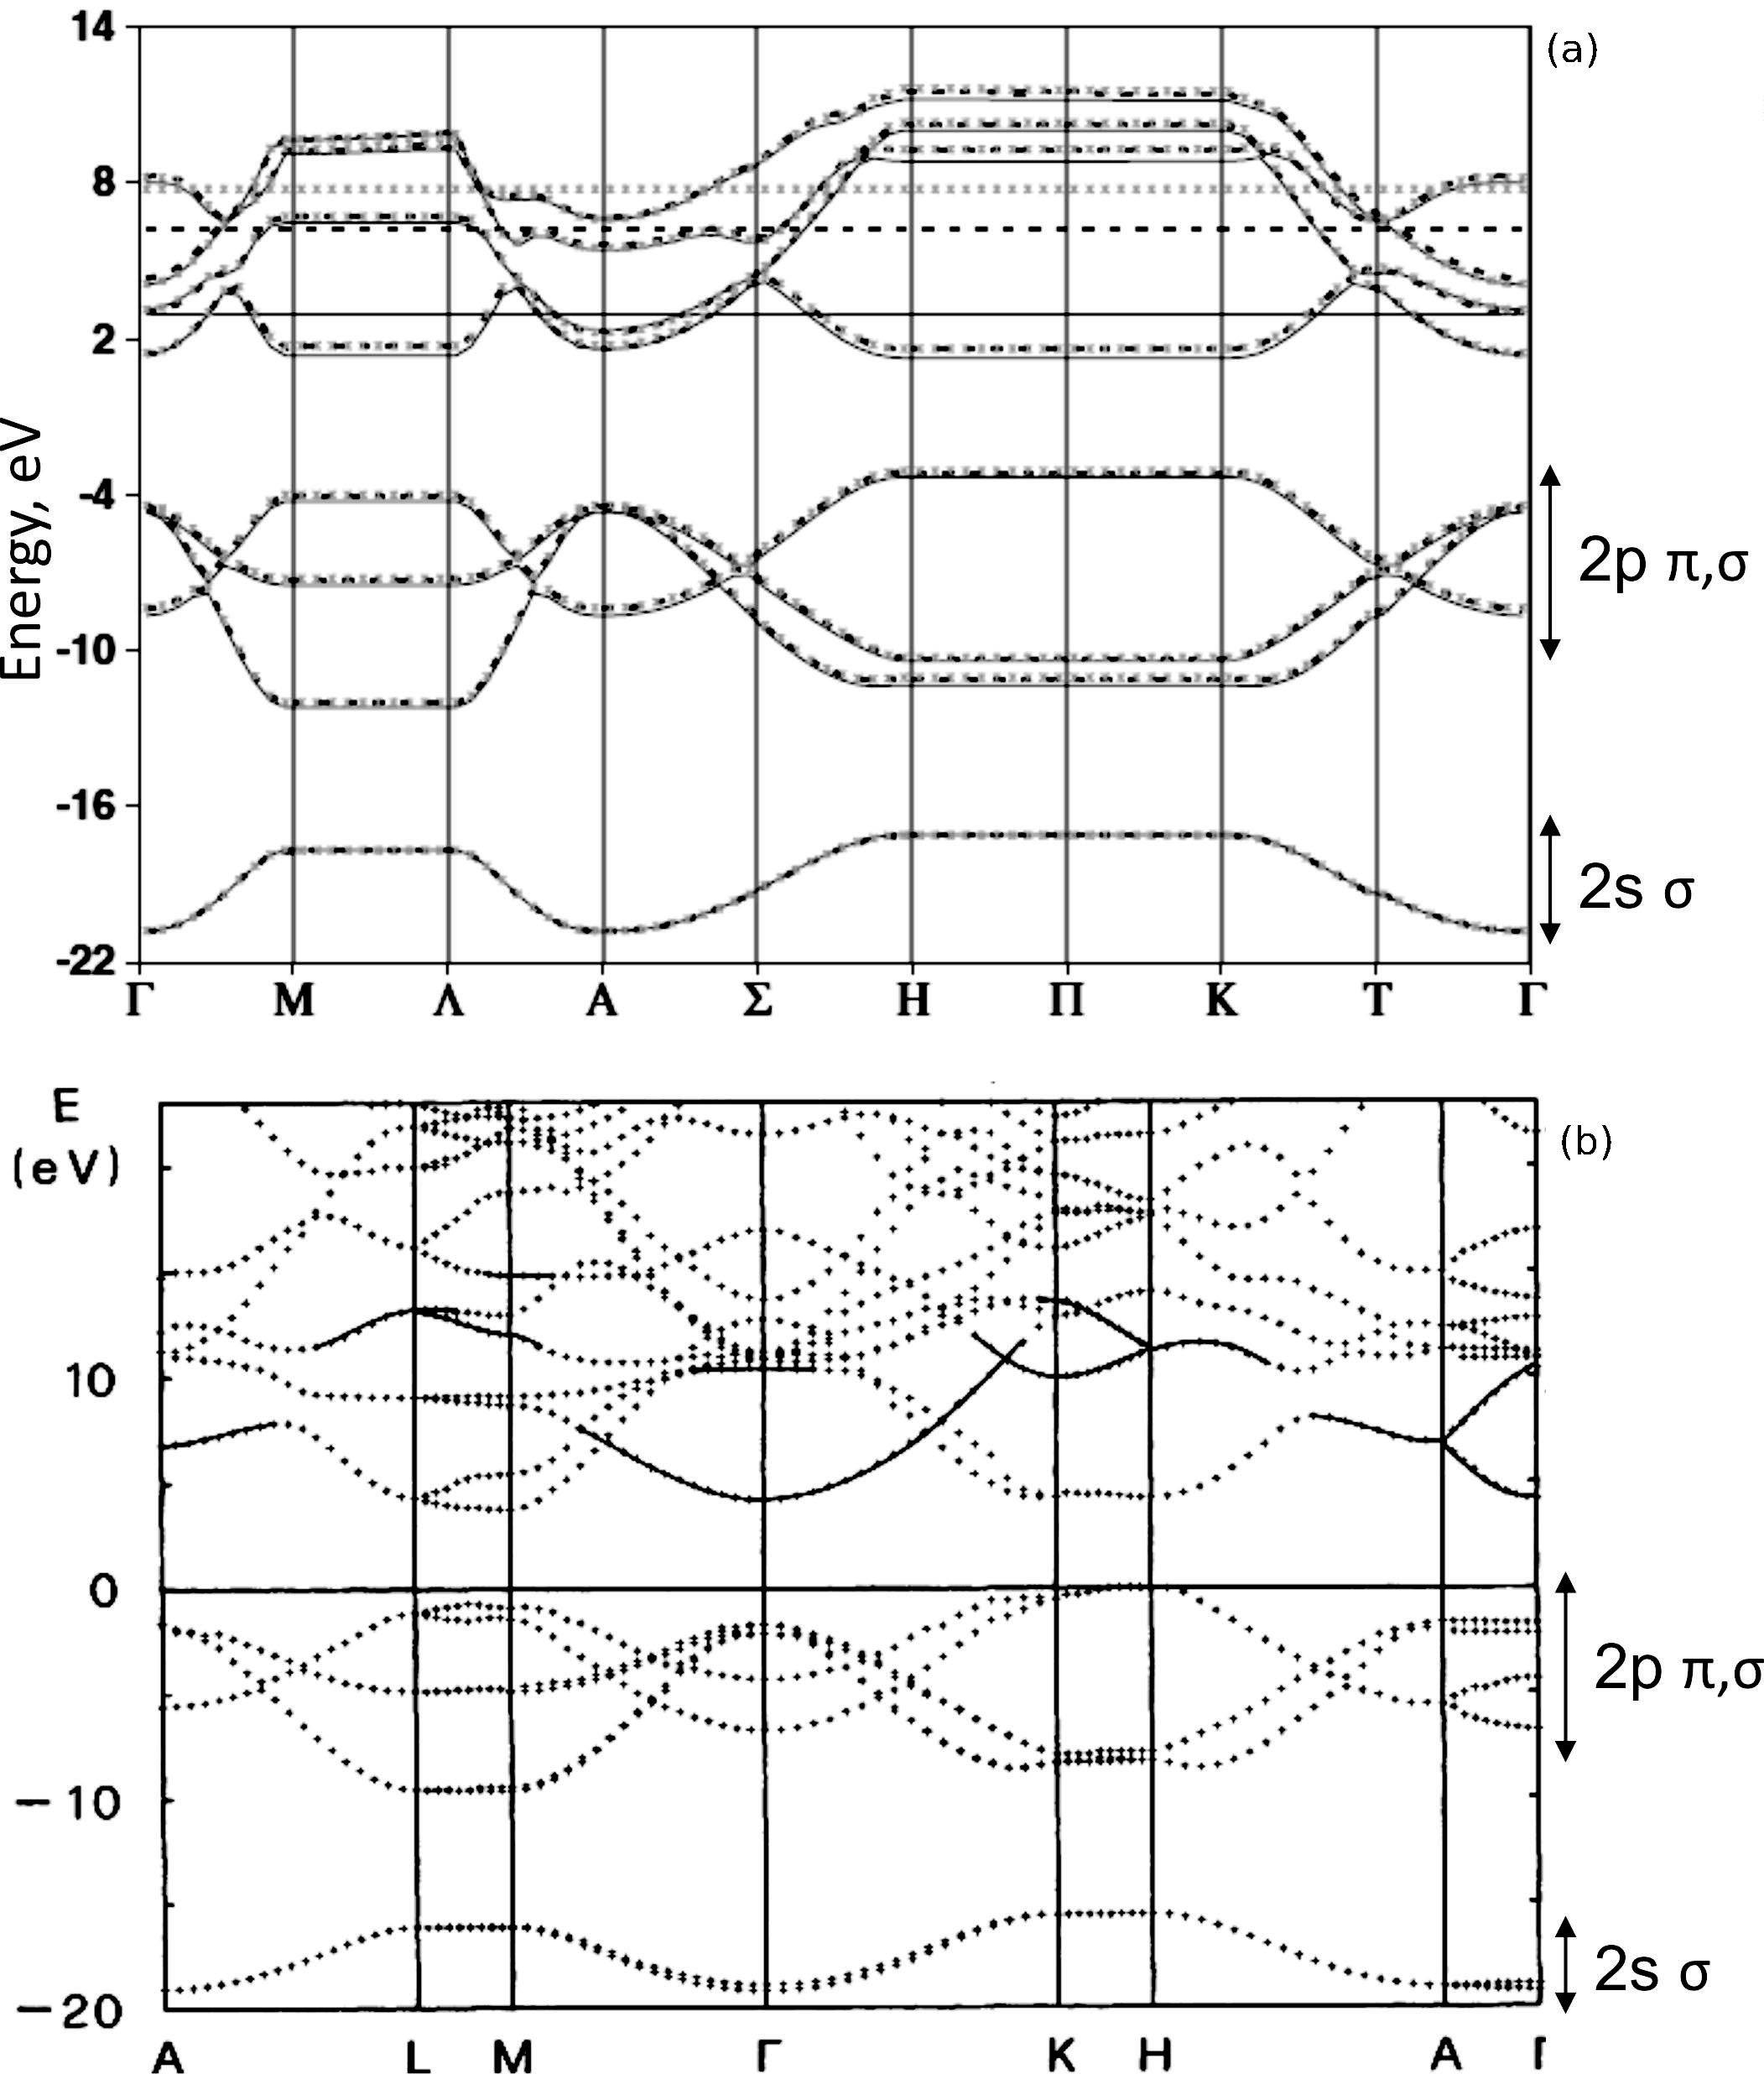
\includegraphics[width=0.6\linewidth]{BN_electron_structure.png}}
\caption{Электронная структура монослоя (а) и многослойного (объемного) (b)
гексагонального нитрида бора~\cite{Ooi2006}.}
\label{pic:BN_electronic_structure}
\end{figure}


Электронная структура как многослойного, так и монослойного h-BN обладает
запрещенной зоной порядка 6~\si{\eV}~\cite{Ooi2006} и имеет похожий вид
рис.~\ref{pic:BN_electronic_structure}. Электронная плотность, в основном,
локализована на атомах азота ввиду их большей электроотрицательности по сравнению с бором~\cite{Grad2003,Catellani1987}. Результатом этого является
сильная ковалентная связь $\mathrm{B-N}$. 
Частично ионный характер связей бора и азота приводит к энергетическому 
разделению свободных и занятых состояний, из-за этого h-BN обладает широкой
запрещенной зоной. 


В спрессованном состоянии h-BN обладает 
полупроводниковыми свойствами, а присутствие примесей в соединении 
может вызывать люминесценцию~\cite{Museur2008}. В связи с этим гексагональный нитрид 
бора интересен областью применения как в цветной металлургии, 
благодаря своей химической инертности и антиадгезионным свойствам по 
отношению к металлам и сплавам, так и в полупроводниковой 
промышленности, благодаря широкой запрещенной зоне~\cite{
Serzhantova2011}.

\section{Приготовление монослоя h-BN на поверхности металла}

Для приготовления монослоя гексагонального нитрида бора на поверхности
переходного
металла обычно используют метод химического осаждения из газообразной фазы
(Chemical Vapor Deposition, CVD). В этом методе материал поступает на 
поверхность подложки в виде газообразных соединений (прекурсора). Молекула 
газа разлагается на горячей поверхности, а ненужные фрагменты молекул
с нее десорбируются. При использовании метода CVD реакции в газовой фазе не 
влияют на рост из-за большой средней длины свободного пробега молекул газа 
при низких давлениях, и рост определяется только химическими реакциями на
поверхности образца. Так как поверхность выращенного образца обычно не
обладает каталитическим свойствами по отношению к прекурсору, то, после
исчезновения свободных участков подложки, скорость реакции заметно 
понижается, а, когда подложка полностью покрывается монослоем, практически
прекращается. Таким образом метод CVD можно считать самопрерывающимся. Этот
метод оказывается идеальным инструментом для получения монослоев на 
поверхности переходных металлов.


В качестве прекурсора для приготовления гексагонального нитрида бора 
используют боразин ($\mathrm{B_3N_3H_6}$)~\cite{Orlando2012}. В настоящей
работе боразин был приготовлен по методу описанному в работе~\cite{Wideman1995}. На рис.~\ref{pic:CVD_BN} проиллюстрировано 
\begin{figure}[!ht]
\center{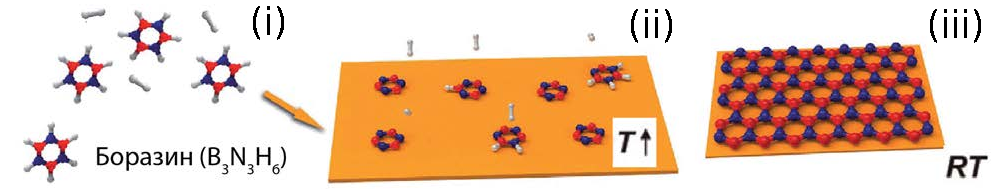
\includegraphics[width=1\linewidth]{CVD_BN.png}}
\caption{Схематическое представление выращивания монослоя гексагонального
нитрида бора на поверхности переходного металла методом CVD.}
\label{pic:CVD_BN}
\end{figure}
схематическое представление выращивания монослоя гексагонального
нитрида бора на поверхности переходного металла методом CVD. Процесс можно 
разбить на 3 основных этапа. На первом этапе (i) в вакуумную камеру напускают
$\mathrm{B_3N_3H_6}$, в которой находится подогреваемая подложка. На втором
этапе (ii) происходит каталитическое термическое разложение молекул прекурсора
в результате его взаимодействия с поверхностью переходного металла. На поверхности остаются только молекулы бора и азота, а
водород десорбируется в газообразном состоянии. Далее молекулы азота и бора
формируют островки на поверхности подложки. Срастаясь между собой, островки
h-BN формируют монослой гексагонального нитрида бора, а каталитическая
реакция прекурсора останавливается -- этап (iii). 



\section{Гексагональный нитрид бора на металлических подложках}

Постоянные решетки гексагонального нитрида бора и металлической подложки
практически всегда различаются, в результате чего происходит изменение
как электронной, так и кристаллической структуры h-BN~\cite{Preobrajenski2007_h-BN_monolayer_on_metals}.
Например, появление суперструктуры муара является известной особенностью
для двумерных материалов. В работе~\cite{FarwickzumHagen2016} 
исследовалась структура 
системы h-BN/Ir(111). Поверхность Ir(111) имеет гексагональную 
кристаллическую структуру, а постоянная решетки ($2.71~\si{\angstrom}$),
что примерно на 8\% превышает постоянную решетки гексагонального нитрида бора.
Разница постоянных решетки подложки и монослоя приводит к образованию 
структуры муара,
\begin{figure}[!ht]
\center{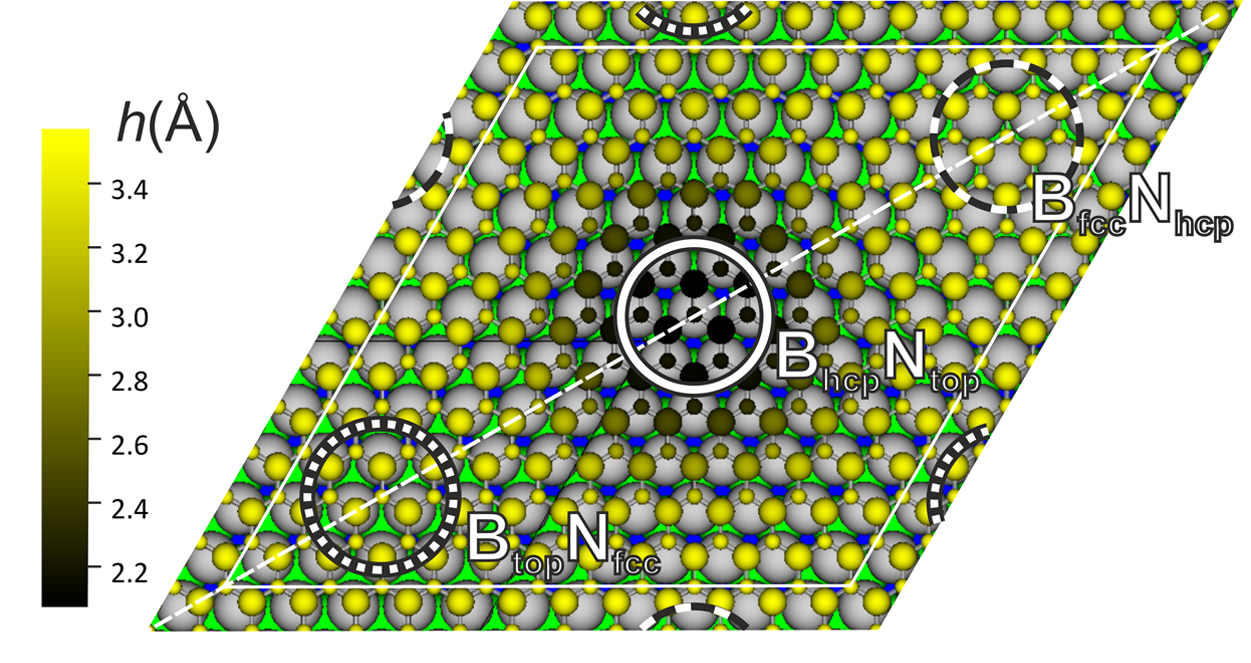
\includegraphics[width=0.7\linewidth]{BN_moir.png}}
\caption{DFT расчет системы h-BN/Ir~\cite{FarwickzumHagen2016}.}
\label{pic:BN_moir}
\end{figure}
а также происходит корругация на поверхности (изменение расстояния от атомов 
монослоя до атомов 
подложки, в зависимости от их взаимного расположения 'top', 'hcp' или 'fcc') 
рис.~\ref{pic:BN_moir}.
Такие сверхструктуры были обнаружены для h-BN на Pt(111)~\cite{Cavar2008},
Ir(111)~\cite{FarwickzumHagen2016,Preobrajenski2008_Adsorption-inducedgapstatesofh-BNonmetalsurfaces,
Usachov2012, Orlando2012},
Ru(0001)~\cite{Brugger2009}, Fe(110)~\cite{Vinogradov2012} и Pd(111)~\cite{Nagashima1995}.


В настоящей работе подложкой для гексагонального нитрида бора являлся Co(0001). Постоянные решетки кобальта и h-BN совпадают с точностью до 0.5\%~\cite{Usachov2018_h-BN/_PED_STM}, это означает, что структуры муара на 
поверхности системы h-BN/Co(0001) не возникает.

\section{Взаимодействие систем h-BN/металл с кислородом}





Одним из наиболее интересных направлений исследования систем graphene/металл и
h-BN/металл является исследование таких структур при взаимодействии с 
кислородом. Кислород является очень агрессивным элементом, особенно в атомарном
виде. Объемный BN оказывается очень химически инертным и не окисляется 
при температурах в несколько сотен градусов~\cite{Li2014}, но при контакте
с металлом его химические свойства могут меняться.
Например, в работе~\cite{Simonov2012_h-BN/Ir_Oxydation} был исследован
процесс окисления интерфейса h-BN/Ir(111) в атомарном кислороде. Авторами
было показано, что при окислении такой структуры происходит два процесса.
Процесс встраивания атомов кислорода в решетку гексагонального нитрида бора,
с последующей десорбцией атомов азота,
и процесс интеркаляции атомов кислорода под монослой h-BN.  
Следствием встраивания атомов кислорода в решетку нитрида бора является 
образование кислород-замещенных структур $\mathrm{BN_{3-x}O_x}(x=1,2,3)$,
причем на первых этапах экспозиции преимущественно появляется структура вида $\mathrm{BN_2O}$, а на последних конфигурации $\mathrm{BNO_2}$ и $\mathrm{BO_3}$.
Также авторы отмечают, что встраивание кислорода в решетку h-BN приводит
к характерной деформации последней. Прогрев до температуры 600\degreeС  интерфейса h-BN/Ir(111) после всех этапов
окисления не приводит к восстановлению системы,
как, например, при окислении graphen/Ir(111) и graphen/Pt(111)~\cite{Vinogradov2011}.
Наоборот, авторы сообщают, что в результате прогрева происходит появление
структур вида $\mathrm{B_2O_3}$, что ведет к полному разрушению монослоя 
гексагонального нитрида бора.


Авторы работы~\cite{Makarova2019_h-BN/Ni_Oxydation} исследовали влияние 
кислорода на систему гексагонального нитрида бора на кривом никеле
h-BN/Ni(111), где показали, что в процессе экспозиции интерфейса в кислороде
происходит ослабление связи между монослоем h-BN и подложкой Ni(111) 
в результате интеркаляции атомов кислорода под монослой. 


В работе~\cite{Huber2015_Oxy_Stab_defffects_in_hBN} были теоретически 
исследованы треугольные дефекты в монослое h-BN на Cu(111). Авторы показали, 
что атомы кислорода способствуют стабилизации таких дефектов. 


Теоретические расчеты окисления монослоя гексагонального нитрида бора
в работе~\cite{Zhao2012} показали, что адсорбция атомов кислорода на 
поверхности монослоя приводит к растяжению химических связей $\mathrm{B-N}$ или
даже к разрыву таких связей. Также авторы утверждают, что, в зависимости
от положения атомов кислорода на поверхности монослоя h-BN, может происходить
формирование кислородных цепочек. Появление таких цепочек может приводить
к разрыву монослоя. Из-за ионной связи $\mathrm{B-N}$ миграция
атомов кислорода может проходить над атомами азота, но является сильно
локализованной, вследствие попадания атомов кислорода в 'ловушку' из трех
атомов бора. 


Таким образом, взаимодействие кислорода с интерфейсами вида h-BN/металл 
оказывается очень интересной темой для исследования. Механизм такого
взаимодействия, как показано выше, для разных конфигураций активно изучается 
учеными, и многие виды интерфейсов h-BN/металл уже хорошо изучены.
Однако, есть и малоизученные, например, h-BN/Co(0001), исследование которого
приведено в настоящей работе. В случае с Co(0001), в отличии от Ir(111),
Ni(111) и других переходных металлов, постоянные решетки гексагонального
нитрида бора и кобальта практически совпадают, а это значит, что структуры 
муара на поверхности h-BN/Co(0001) не возникает. Так же в настоящей работе, в 
отличии от~\cite{Simonov2012_h-BN/Ir_Oxydation}, использовался не атомарный, а 
молекулярный кислород, который оказывается менее агрессивным. 















